\section{Phụ lục kết quả đo và bằng chứng thực
thi}\label{phux1ee5-lux1ee5c-kux1ebft-quux1ea3-ux111o-vuxe0-bux1eb1ng-chux1ee9ng-thux1ef1c-thi}

Các bảng dưới được dựng trực tiếp từ CSV/JSON của lần chạy đầy đủ. Mọi
mean cấu hình là trung bình qua năm seed 11, 22, 33, 44, 55; SD dùng
ddof=1. Các ảnh là biểu đồ vẽ từ dữ liệu episode thực thi, không phải
ảnh minh họa sinh bằng mô hình.

\subsection{Bảng tổng hợp thí nghiệm alpha và
epsilon}\label{bux1ea3ng-tux1ed5ng-hux1ee3p-thuxed-nghiux1ec7m-alpha-vuxe0-epsilon}

{\def\LTcaptype{none} % do not increment counter
\begin{longtable}[]{@{}llllll@{}}
\toprule\noalign{}
Cấu hình & Train mean & Eval mean & SD & CI95 ± & Discount (\%) \\
\midrule\noalign{}
\endhead
\bottomrule\noalign{}
\endlastfoot
baseline & 33.6513 & 34.0997 & 1.3678 & 1.6981 & 16.16 \\
alpha\_001 & 32.0944 & 33.6484 & 2.1286 & 2.6425 & 19.91 \\
alpha\_050 & 31.8520 & 31.9533 & 4.1613 & 5.1661 & 38.08 \\
epsilon\_005 & 32.9458 & 33.3973 & 1.6126 & 2.0020 & 27.90 \\
epsilon\_030 & 30.8822 & 31.4300 & 3.9272 & 4.8755 & 33.88 \\
\end{longtable}
}

\subsection{So sánh công bằng với cùng đối
thủ}\label{so-suxe1nh-cuxf4ng-bux1eb1ng-vux1edbi-cuxf9ng-ux111ux1ed1i-thux1ee7}

{\def\LTcaptype{none} % do not increment counter
\begin{longtable}[]{@{}lll@{}}
\toprule\noalign{}
Focal policy & Mean reward/step & SD giữa seed \\
\midrule\noalign{}
\endhead
\bottomrule\noalign{}
\endlastfoot
RL & 34.0997 & 1.3678 \\
Rule & 35.1295 & 0.1261 \\
Never & 35.1295 & 0.1261 \\
Always & 24.9722 & 0.0701 \\
DP & 35.1295 & 0.1261 \\
\end{longtable}
}

\subsection{Thí nghiệm biến đổi discount
40\%}\label{thuxed-nghiux1ec7m-biux1ebfn-ux111ux1ed5i-discount-40}

{\def\LTcaptype{none} % do not increment counter
\begin{longtable}[]{@{}lll@{}}
\toprule\noalign{}
Policy & Mean reward/step & SD giữa seed \\
\midrule\noalign{}
\endhead
\bottomrule\noalign{}
\endlastfoot
frozen\_RL & 32.6415 & 3.3620 \\
retrained\_RL & 33.6009 & 3.3403 \\
Rule & 35.1295 & 0.1261 \\
DP & 35.1295 & 0.1261 \\
\end{longtable}
}

\subsection{Q-table minh họa seed
42}\label{q-table-minh-hux1ecda-seed-42}

{\def\LTcaptype{none} % do not increment counter
\begin{longtable}[]{@{}
  >{\raggedright\arraybackslash}p{(\linewidth - 8\tabcolsep) * \real{0.2000}}
  >{\raggedright\arraybackslash}p{(\linewidth - 8\tabcolsep) * \real{0.2000}}
  >{\raggedright\arraybackslash}p{(\linewidth - 8\tabcolsep) * \real{0.2000}}
  >{\raggedright\arraybackslash}p{(\linewidth - 8\tabcolsep) * \real{0.2000}}
  >{\raggedright\arraybackslash}p{(\linewidth - 8\tabcolsep) * \real{0.2000}}@{}}
\toprule\noalign{}
\begin{minipage}[b]{\linewidth}\raggedright
Demand
\end{minipage} & \begin{minipage}[b]{\linewidth}\raggedright
Opponent previous
\end{minipage} & \begin{minipage}[b]{\linewidth}\raggedright
Q(no discount)
\end{minipage} & \begin{minipage}[b]{\linewidth}\raggedright
Q(discount)
\end{minipage} & \begin{minipage}[b]{\linewidth}\raggedright
Greedy action
\end{minipage} \\
\midrule\noalign{}
\endhead
\bottomrule\noalign{}
\endlastfoot
0 & 0 & 184.212867 & 199.449036 & 1 \\
0 & 1 & 221.956047 & 181.668010 & 0 \\
1 & 0 & 227.279761 & 235.197513 & 1 \\
1 & 1 & 197.471701 & 218.162589 & 1 \\
\end{longtable}
}

\subsection{Từng seed của
baseline}\label{tux1eebng-seed-cux1ee7a-baseline}

{\def\LTcaptype{none} % do not increment counter
\begin{longtable}[]{@{}llll@{}}
\toprule\noalign{}
Seed & RL mean & Rule mean cùng tape & RL discount (\%) \\
\midrule\noalign{}
\endhead
\bottomrule\noalign{}
\endlastfoot
11 & 35.1825 & 35.1825 & 0.00 \\
22 & 32.5267 & 35.0910 & 40.70 \\
33 & 32.6863 & 35.2710 & 40.12 \\
44 & 34.9350 & 34.9350 & 0.00 \\
55 & 35.1680 & 35.1680 & 0.00 \\
\end{longtable}
}

\subsection{Cặp learner trong
self-play}\label{cux1eb7p-learner-trong-self-play}

{\def\LTcaptype{none} % do not increment counter
\begin{longtable}[]{@{}llll@{}}
\toprule\noalign{}
Seed & Learner & Eval mean & Discount (\%) \\
\midrule\noalign{}
\endhead
\bottomrule\noalign{}
\endlastfoot
11 & 0 & 30.5514 & 19.64 \\
11 & 1 & 32.5935 & 40.21 \\
22 & 0 & 35.0545 & 0.00 \\
22 & 1 & 35.1300 & 0.00 \\
33 & 0 & 35.3565 & 0.00 \\
33 & 1 & 35.4800 & 0.00 \\
44 & 0 & 34.8160 & 0.00 \\
44 & 1 & 34.7835 & 0.00 \\
55 & 0 & 34.8630 & 0.00 \\
55 & 1 & 35.0500 & 0.00 \\
\end{longtable}
}

\subsection{Đối chiếu bản gốc và bản mở rộng seed
42}\label{ux111ux1ed1i-chiux1ebfu-bux1ea3n-gux1ed1c-vuxe0-bux1ea3n-mux1edf-rux1ed9ng-seed-42}

Cùng seed số học không tạo cùng chuỗi khi cách dùng RNG khác. Bảng này
ghi hai protocol riêng; không lấy chênh lệch làm bằng chứng chất lượng
một thuật toán khác.

{\def\LTcaptype{none} % do not increment counter
\begin{longtable}[]{@{}lll@{}}
\toprule\noalign{}
Protocol & Focal mean & Opponent mean \\
\midrule\noalign{}
\endhead
\bottomrule\noalign{}
\endlastfoot
Code gốc nguyên văn & 35.1275 & 34.9685 \\
Bản mở rộng, split RNG & 25.5591 & 24.6856 \\
\end{longtable}
}

\begin{center}
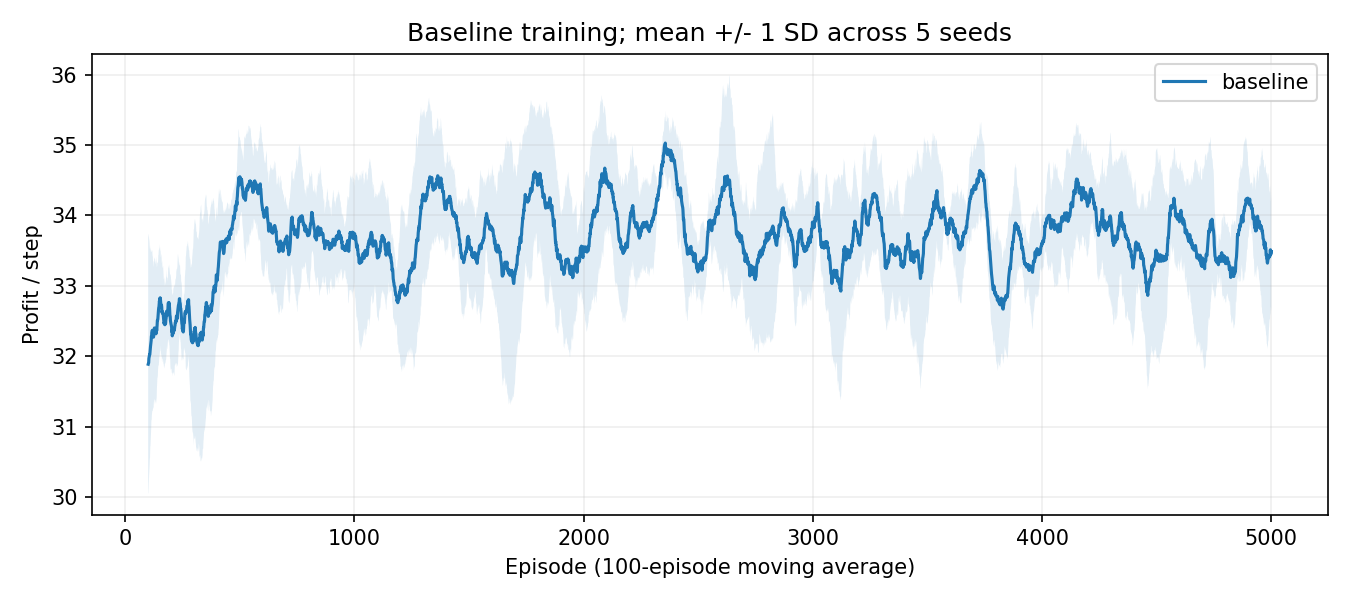
\includegraphics[width=0.98\linewidth]{results/assignment/learning_curve.png}
\captionof{figure}{Learning curve baseline: moving average 100 episode, mean và một SD qua năm seed.}
\end{center}

\begin{center}
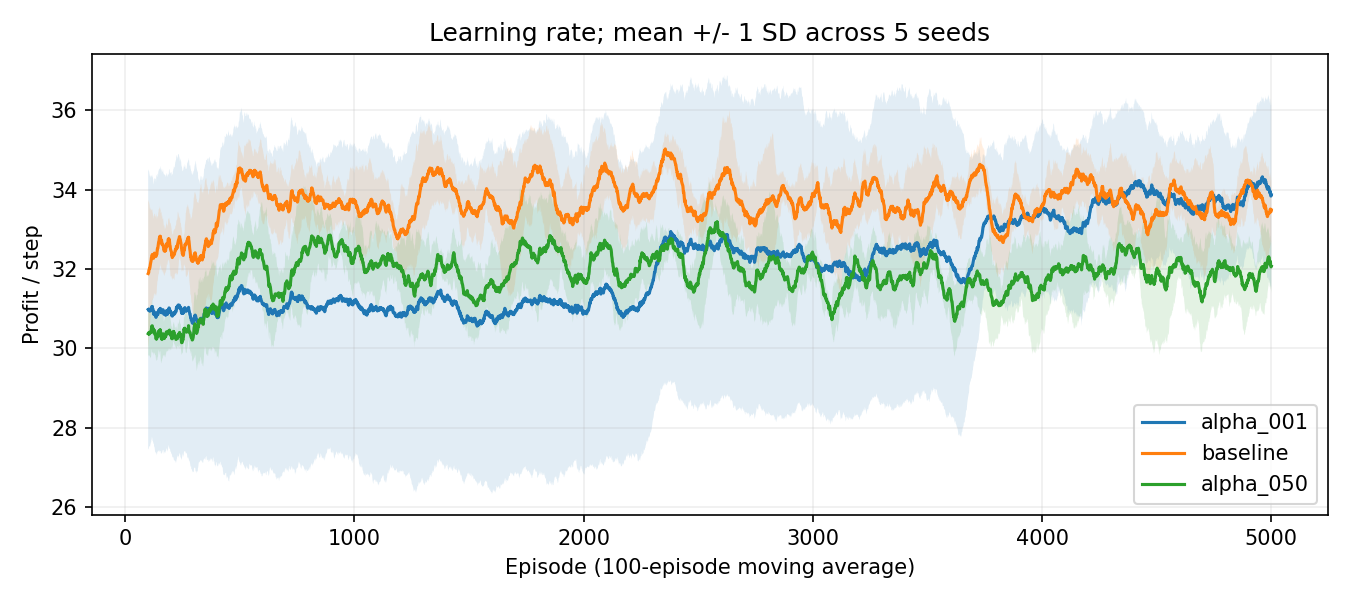
\includegraphics[width=0.98\linewidth]{results/assignment/learning_rates.png}
\captionof{figure}{So sánh ba learning rate với cùng epsilon schedule.}
\end{center}

\begin{center}
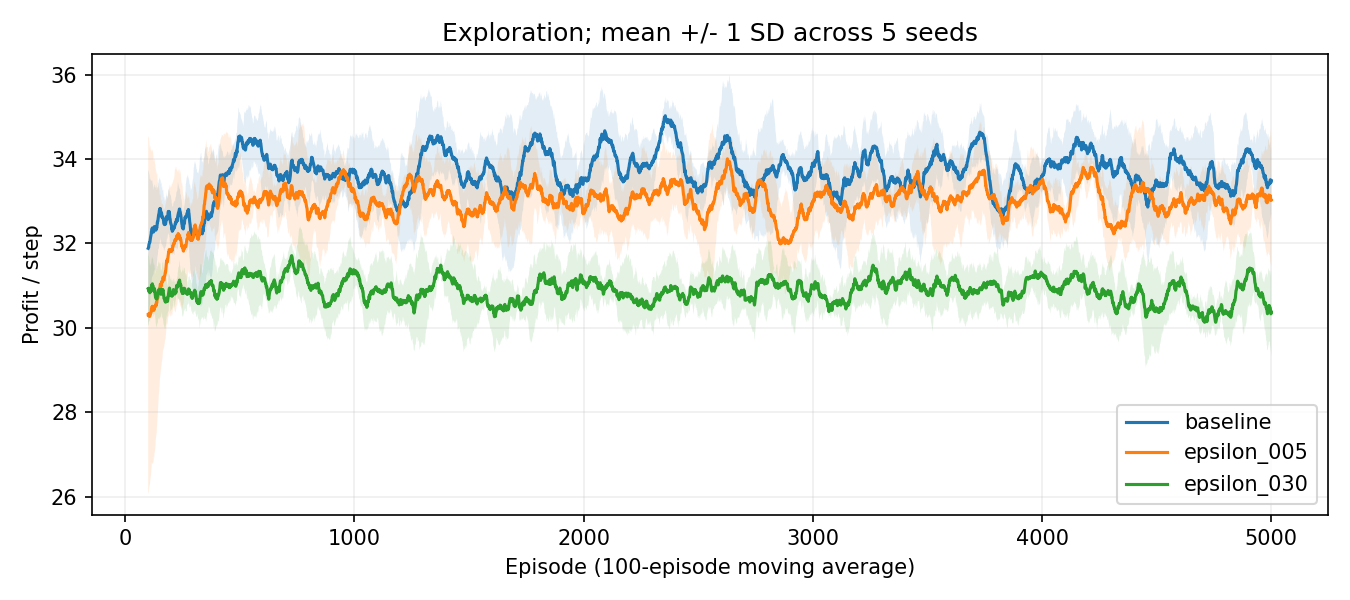
\includegraphics[width=0.98\linewidth]{results/assignment/exploration.png}
\captionof{figure}{So sánh ba cấu hình epsilon; mọi cấu hình đánh giá với epsilon bằng 0.}
\end{center}

\begin{center}
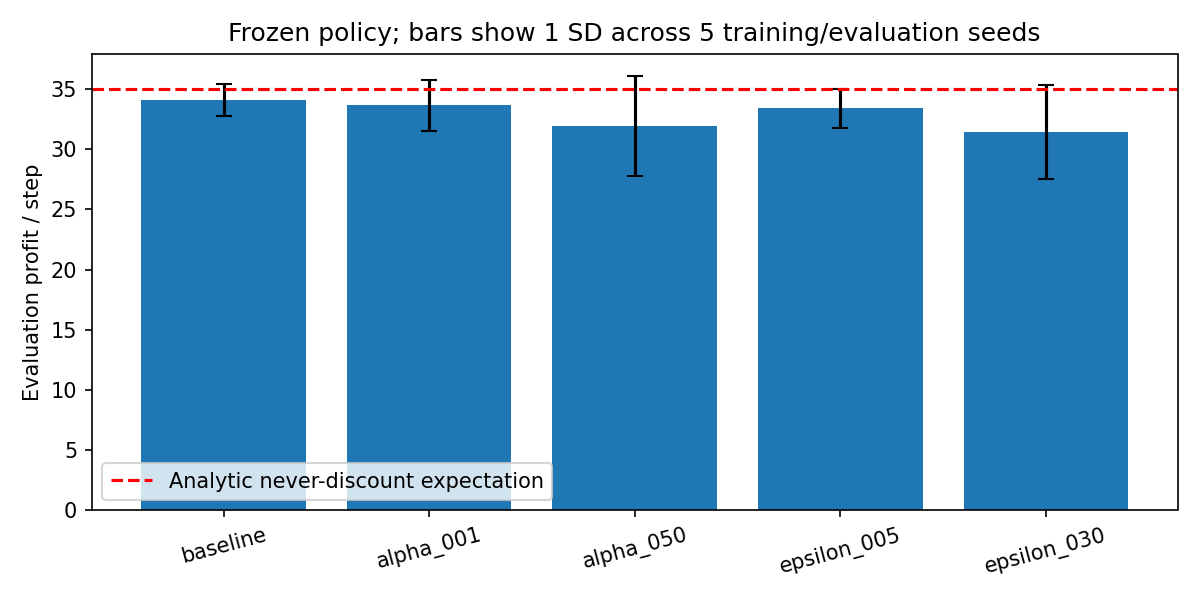
\includegraphics[width=0.98\linewidth]{results/assignment/evaluation.png}
\captionof{figure}{Policy đóng băng: mean và SD giữa seed; đường 35 là kỳ vọng lý thuyết.}
\end{center}

\begin{center}
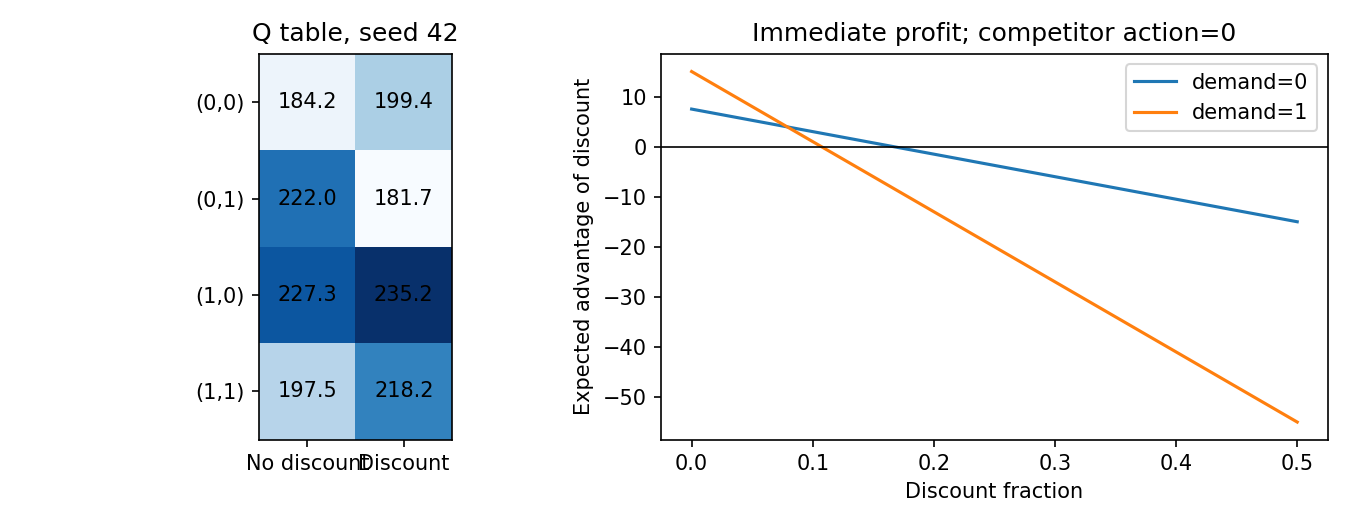
\includegraphics[width=0.98\linewidth]{results/assignment/q_and_sensitivity.png}
\captionof{figure}{Q-table seed 42 và độ nhạy lợi nhuận tức thời theo discount fraction.}
\end{center}

\subsection{Mã Python cốt lõi}\label{muxe3-python-cux1ed1t-luxf5i}

Đây là các đoạn mã được lấy trực tiếp từ nguồn đã thực thi. Tệp đầy đủ
và bản tham chiếu có trong thư mục assignment; các đoạn bên dưới đủ để
kiểm cách cập nhật, tách evaluation và tính oracle.

\lstinputlisting[firstline=60,lastline=73,caption={Q-learning và luật, trích từ mã chạy}]{assignment/agent02_experiment.py}
\lstinputlisting[firstline=106,lastline=118,caption={Quy hoạch động hữu hạn chân trời}]{assignment/agent02_experiment.py}
\lstinputlisting[firstline=120,lastline=149,caption={Đánh giá đóng băng với common random numbers}]{assignment/agent02_experiment.py}

\subsection{Bằng chứng kiểm
thử}\label{bux1eb1ng-chux1ee9ng-kiux1ec3m-thux1eed}

Bộ kiểm thử assignment có 12 ca, đã chạy thành công. Các ca kiểm công
thức ví dụ 4.65; terminal không bootstrap; observation sau joint action;
từ chối action sai; margin; bảng luật; Q không đổi khi đánh giá; tổng
action counts; tái lập evaluation; DP chọn không giảm; tái lập training;
và sample mean gần kỳ vọng 35 khi số episode lớn.

\begin{verbatim}
python3 -m unittest discover -s assignment -p 'test_*.py'
............
Ran 12 tests
OK
\end{verbatim}

Log thực tế được giữ trong build/assignment\_tests.log. Thời lượng đo cụ
thể phụ thuộc máy, nên không dùng thời lượng test làm chỉ số thuật toán.
Mười hai test không chứng nhận mô hình kinh tế đúng ngoài thực tế; chúng
kiểm những bất biến quan trọng của implementation.
